\section{Task 1, DC-motor}

% Task A
\subsection{Task A}
\textbf{\textit{Task: Find the poles of the system.}}
\newline
\textit{Code: \ref{apx:1A_matlab}}
The below equation is the transfer function of the system. It shows that it is a second order system and therefore has two poles. 

\begin{equation}
    sys = \frac{1.414}{s^2 + 5 s + 6}
\end{equation}

The MATLAB code in appendix \ref{apx:1A_matlab} was used to find the poles of the system. The answer was cross-checked by plotting the Root locus script. The following output was given by MATLAB.

\begin{align*}
    P1 = -3.0000 \\
    P2 = -2.0000
\end{align*}

\begin{figure}[h]
    \centering
    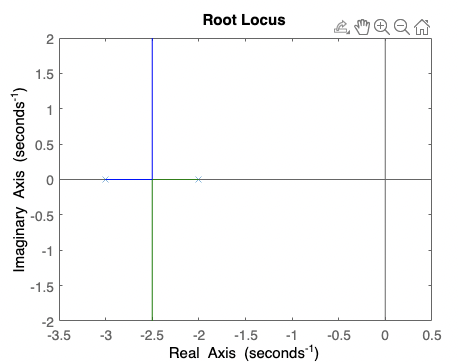
\includegraphics[width = 0.6\textwidth]{Images/1A_RLocus.png}
    \caption{Root locus of DC-motor}
    \label{fig:1A RLocus}
\end{figure}

The poles are located in (-2,0) and (-3,0). This means that the system is stable.

%Task B
\subsection{Task B}
\textbf{\textit{Task: Find the centroid of the system.}}

The centroid of the system can be found in the middle of the poles and it is highlighted in the root locus plot in Figure \ref{fig:1A RLocus}.
The centroid is given by $\frac{\sum Poles - \sum Zeros}{n - m}$ where n is numerator and m is denominator. In this case the calculation will be as simple as $\frac {(-2) + (-3)}{2}$ which equals -2.5. \\
The centroid is located at (-2.5, 0).

%Task C
\subsection{Task C}
\textbf{\textit{Task: Plot the step response of the unity feedback system.}}
\newline
\textit{Code: \ref{apx:1C_matlab}}
The plot in Figure \ref{fig:1C_StepResponse} was output of the referenced code.

\begin{figure}[h]
    \centering
    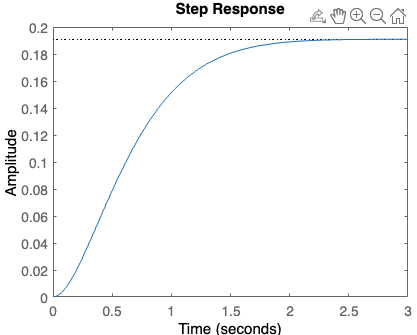
\includegraphics[width = 0.6\textwidth]{Images/1C_Step.png}
    \caption{Step response of system with feedback.}
    \label{fig:1C_StepResponse}
\end{figure}

%Task D
\subsection{Task D}
\textbf{\textit{Task: Design a PI controller to eliminate the steady state error with allowable overshoot less than 10 \%. }}
\newline
\textit{Code: \ref{apx:1D_matlab}}

When designing a PI controller you need a Kp- and a Ki value while the Kd value will be 0. An educated guess of the parameters was made. Ki = 1 and Kp = 5.
The PI controller can be seen in equation \ref{fig:PI}.

\begin{equation}
    G = \frac{s + 5}{s}
    \label{fig:PI}
\end{equation}



\begin{equation}
    TF = \frac{G(s)}{1+G(s)} = \frac{\frac{n}{m}}{1+\frac{n}{m}} = \frac{n(s)}{m(s)+n(s)}
\end{equation}

\begin{figure}[h!]
    \centering
    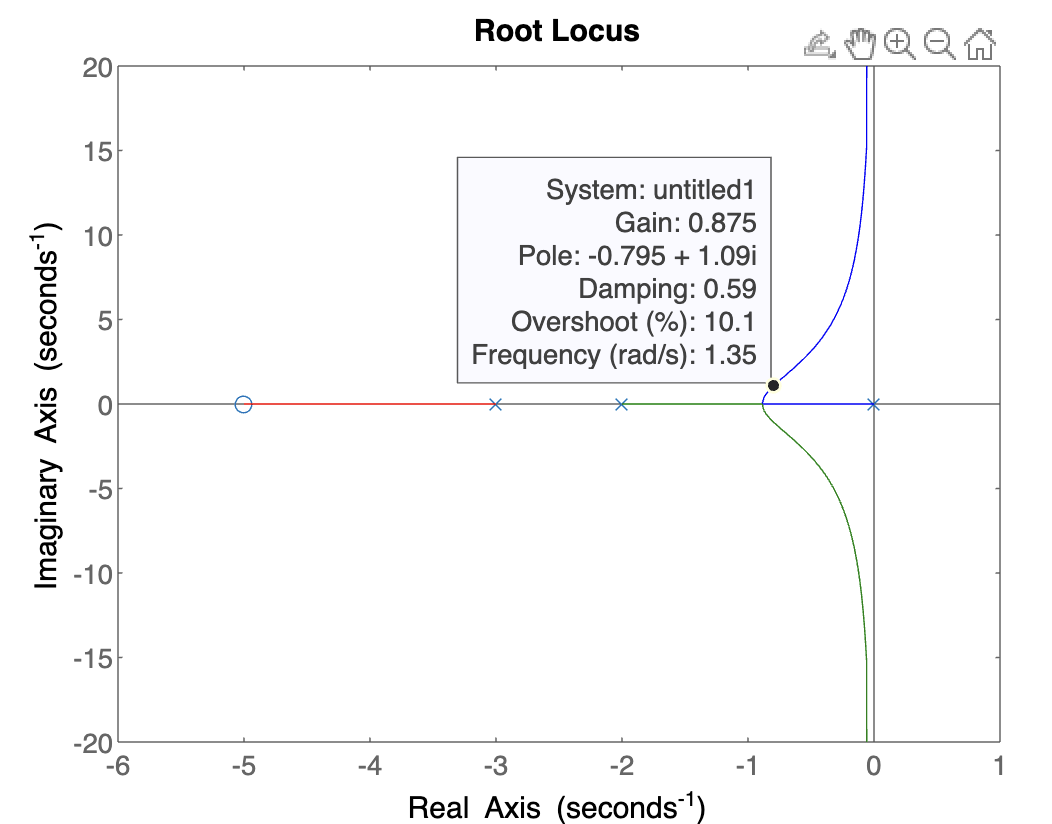
\includegraphics[width = 0.6\textwidth]{Images/1D_Rlocus.png}
    \caption{Step response of system with PI and feedback.}
    \label{fig:1D_Rlocus}
\end{figure}

The root locus gave a gain of 0.875 for a desired 10 \% overshoot. With the following configuration the system met the criteria given in the task.

\begin{figure}[h!]
    \centering
    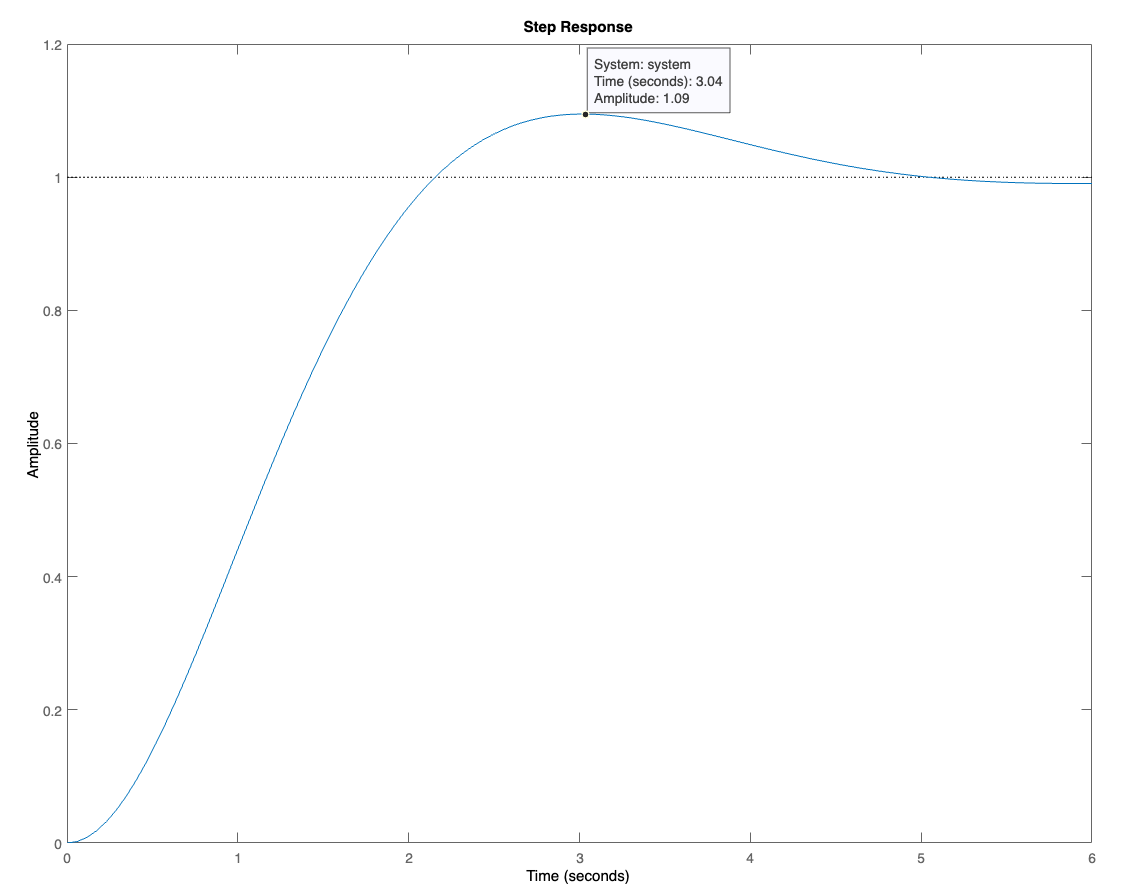
\includegraphics[width = 0.6\textwidth]{Images/1D_Step.png}
    \caption{Step response of system with PI and feedback.}
    \label{fig:1D_Step}
\end{figure}

\newpage
%Task E
\subsection{Task E}
\textbf{\textit{Task: Design a lead compensator such that the root locus passes through (-3+i) and (-3-i).}}
\newline
\textit{Code: \ref{apx:1E_matlab}}

\begin{equation}
    \sum Poles \angle - \sum Zeros \angle = 180\degree \\
\end{equation}

Assuming that the zero is located in -4, we can calculate the new pole of the system. The angles were calculated using trigonometry.

\begin{figure}[h!]
    \centering
    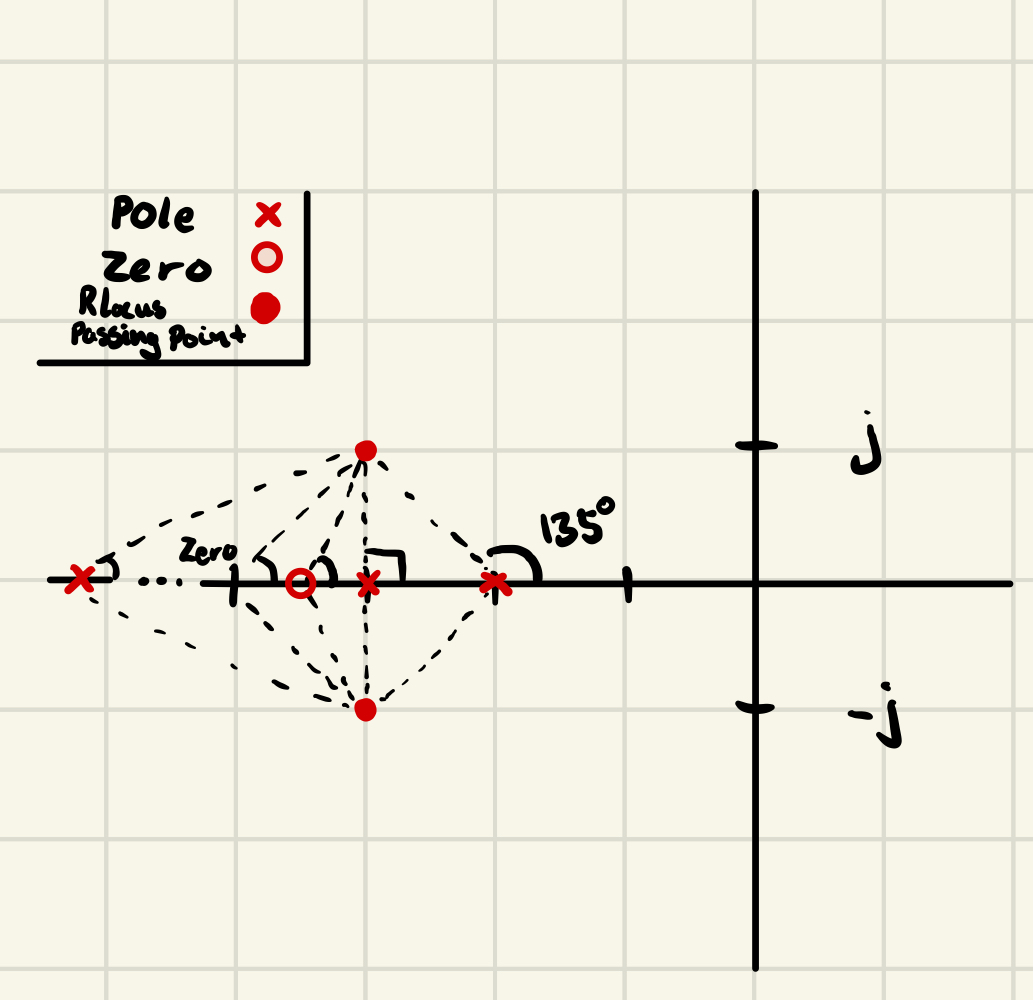
\includegraphics[width = 0.6\textwidth]{Images/1E_Plot.jpeg}
    \caption{Scetch of 1E problem}
    \label{fig:1E_Plot}
\end{figure}


\begin{center}
\begin{tabular}{c c}
    $`\sum Poles \angle = 90 \degree + 135 \degree$ & $\sum Zeros \angle = \arctan (\frac{1}{1})$ \\
    $`\sum Poles \angle = 225 \degree $ & $\sum Zeros \angle = 63.43 \degree$\\
\end{tabular}
\end{center}

\begin{center}
    $\sum = 225 \degree - 63.43 \degree$ \\ 
    $\sum = 161.57$ \\
    $Pole = 180 \degree - 161.57 \degree = 18.43 \degree$ \\
    $\frac{1}{\tan (18.43)} = 3$ \\
    $-3 - 3 = -6$
   %$\lim_{angle \to 0} Pole \approx SmallAngle $
\end{center}

This means that the last pole is set to be located in (-6,0).
This results in the following lead compensator:
\begin{equation}
    LC = \frac{s+3.5}{s+6}
\end{equation}

\begin{figure}[h!]
    \centering
    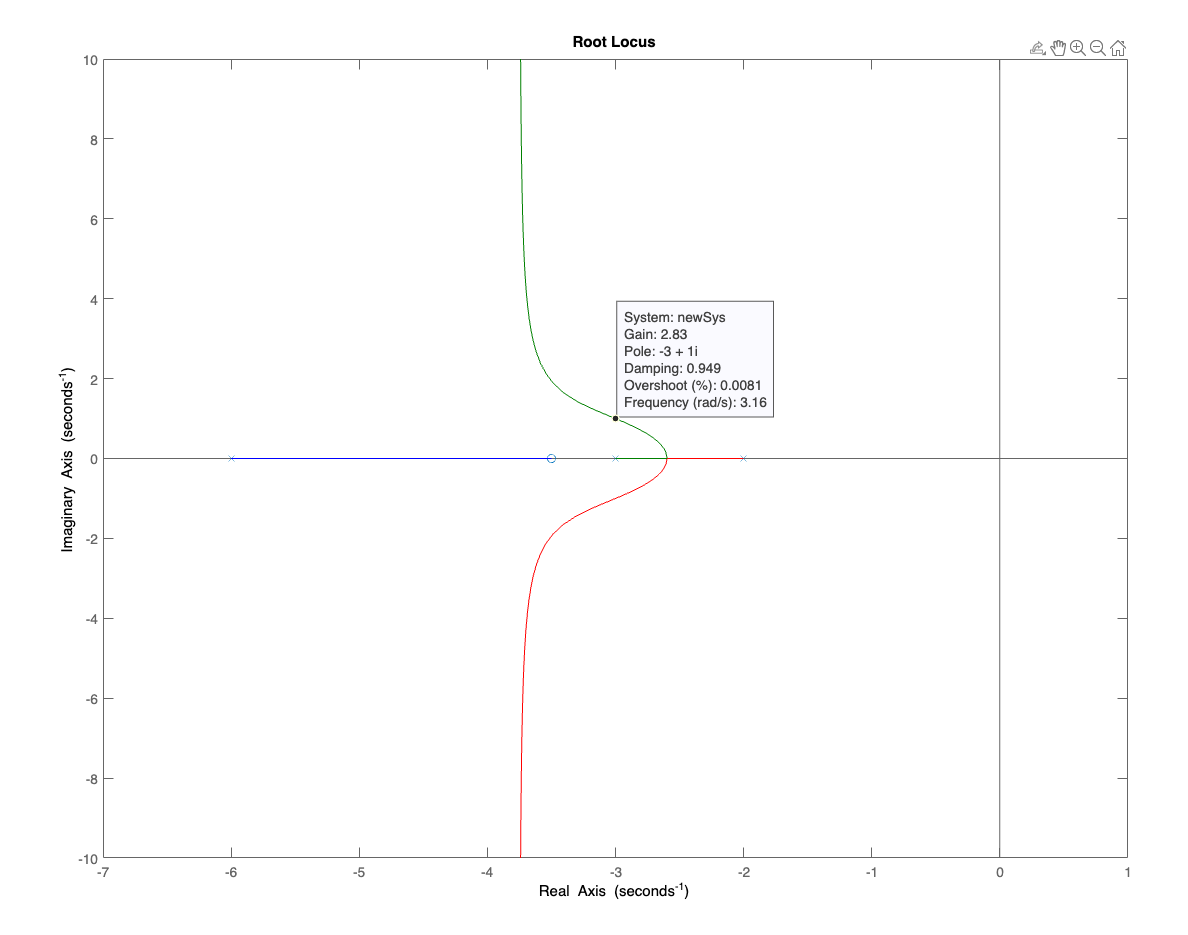
\includegraphics[width = 0.6\textwidth]{Images/1E_Rlocus.png}
    \caption{Rlocus of the original transfer function multiplied by the designed lead compensator}
    \label{fig:1E_Rlocus}
\end{figure}

%Task F
\subsection{Task F}
\textbf{\textit{Task:  Plot the step response of (e) (likely you still have steady state error).}}
\newline
\textit{Code: \ref{apx:1F_matlab}}

The system has a steady state at 0.14. 
\begin{figure}[h!]
    \centering
    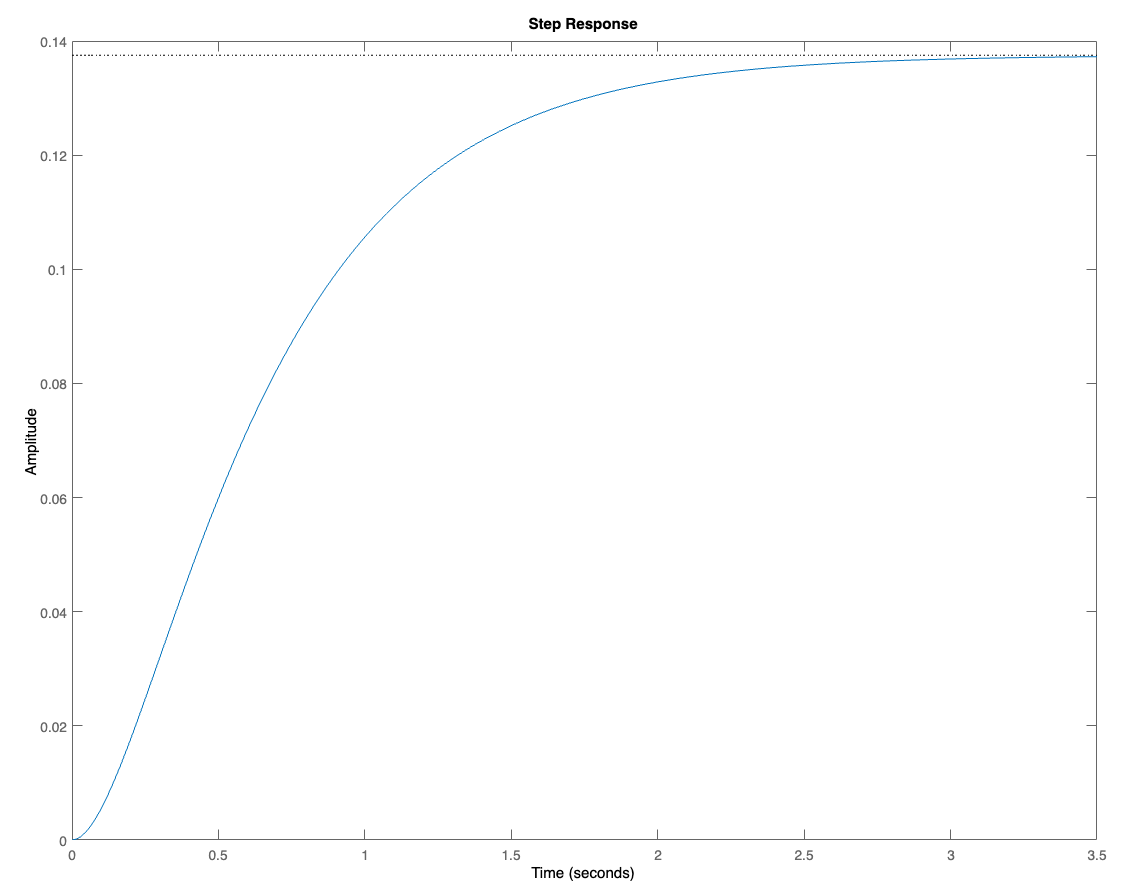
\includegraphics[width = 0.6\textwidth]{Images/1F_Step.png}
    \caption{Step response of system with lead compensator.}
    \label{fig:1E_Step}
\end{figure}

%Task G
\subsection{Task G}
\textbf{\textit{Task: Calculate the DC gain ($K_{DC}$) of the closed-loop system using the following formula:}}

\begin{equation}
    K_{DC} = \lim_{s \to 0} G(s)
\end{equation}

\textbf{\textit{where G(s) is the transfer function of the closed-loop system. The pre-compensation is given
by $\overline{N} = \frac{1}{K_{DC}}$.}}

Setting s $\to$ 0 gives the result $K_{DC} = \frac{\sqrt{2}}{6+\sqrt{2}}$.\\
The pre-compensation is given by $\overline{N} = \frac{1}{K_{DC}} \implies \overline{N} = \frac{6+\sqrt{2}}{\sqrt{2}}$

%Task H
\subsection{Task H}
\textbf{\textit{Task: Multiply the pre-compensation with the input and plot the result.}}
\newline
\textit{Code: \ref{apx:1H_matlab}}

\begin{figure}[h!]
    \centering
    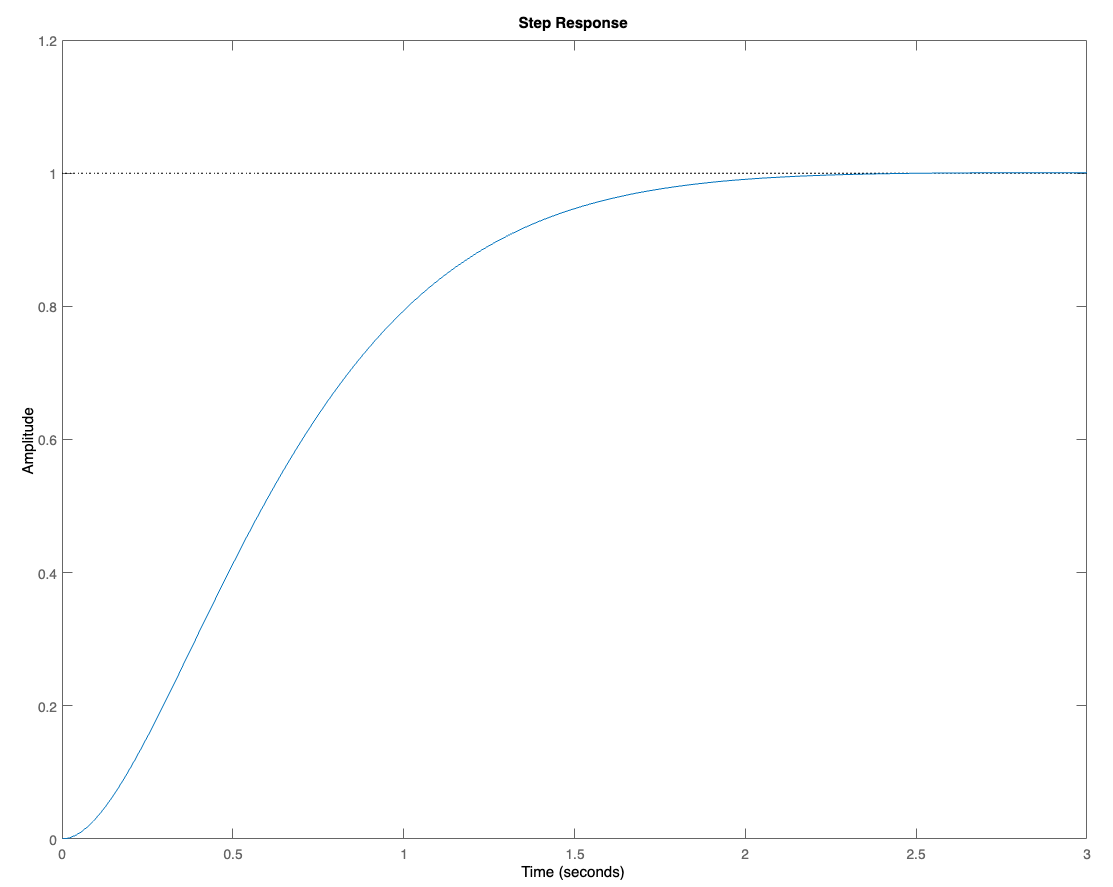
\includegraphics[width = 0.6\textwidth]{Images/1H_Step.png}
    \caption{Step response of system with pre-compensation.}
    \label{fig:1H_Step}
\end{figure}